\documentclass[12pt,a4paper]{scrartcl}
    \usepackage[utf8]{inputenc}
    \usepackage{amsmath}
    \usepackage{amsfonts}
    \usepackage{amssymb}
    \usepackage{graphicx}

    \usepackage[bottom = 1in, left = 0.5in, right = 0.5in, top = 1in]{geometry}

    \usepackage[english]{babel}
    \usepackage[autostyle]{csquotes}
    \usepackage{mathptmx}

    \usepackage[labelfont=bf]{caption}

    \usepackage[default, scale=0.95]{opensans}

    \usepackage[T1]{fontenc}

	\usepackage{fixltx2e}
	
	\usepackage{textcomp}

    % \addto\captionsenglish{\renewcommand{\figurename}{Supplementary Fig.}}
    % \addto\captionsenglish{\renewcommand{\tablename}{Supplementary Table}}

    \title{Figures}
    \date{}

\begin{document}
\maketitle

Note that all figures are scaled by a factor of 2 for display.

\begin{figure}[h]
	\centering
	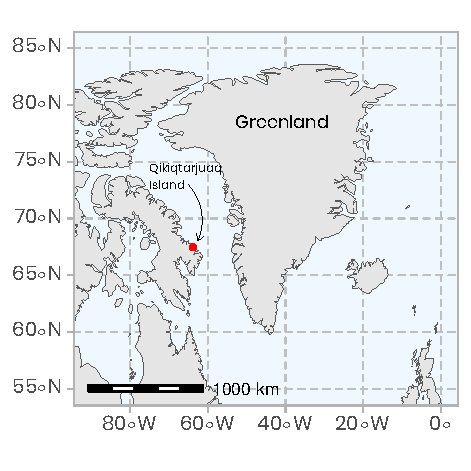
\includegraphics[scale = 2]{../../../graphs/fig1.pdf}
	\caption{Location of the ice camp in the Baffin Bay (red dot) along with the bathymetry.}
\end{figure}

\clearpage
\newpage

\begin{figure}[h]
	\centering
	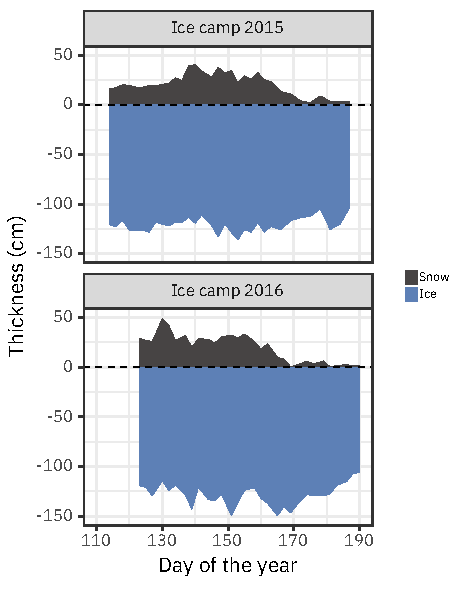
\includegraphics[scale = 2]{../../../graphs/fig2.pdf}
	\caption{Temporal evolution of the snow and sea-ice thickness for both ice camp missions. The dashed horizontal line represents the snow/ice interface.}
\end{figure}

\clearpage
\newpage

\begin{figure}[h]
	\centering
	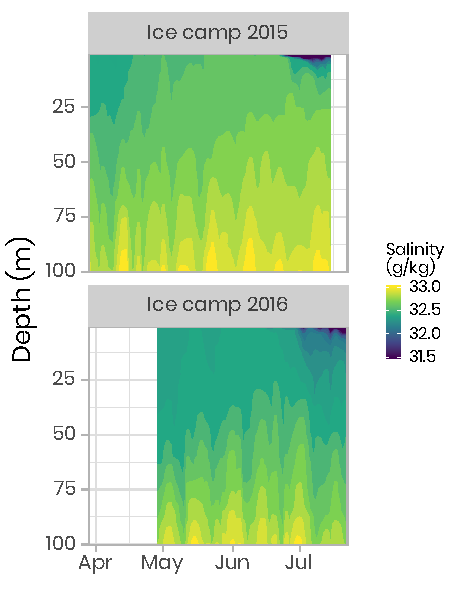
\includegraphics[scale = 2]{../../../graphs/fig3.pdf}
	\caption{Salinity.}
\end{figure}

\begin{figure}[h]
	\centering
	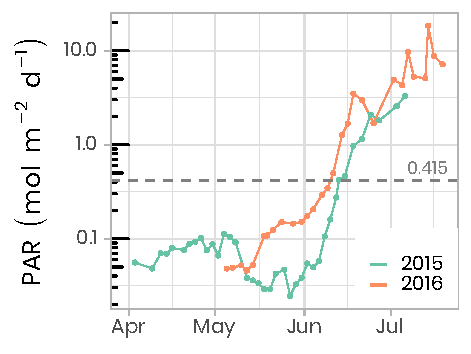
\includegraphics[scale = 2]{../../../graphs/fig4.pdf}
	\caption{Temporal evolution of daily photosynthetically available radiation (PAR) at the sea-ice/water interface (1.3 m depth) for both ice camp missions. The horizontal dashed line show the 0.415 mol photons m\textsuperscript{-2} s\textsuperscript{-1} threshold often used in the literature as the minimum light requirement for primary production.}
\end{figure}

\clearpage
\newpage

\begin{figure}[h]
	\centering
	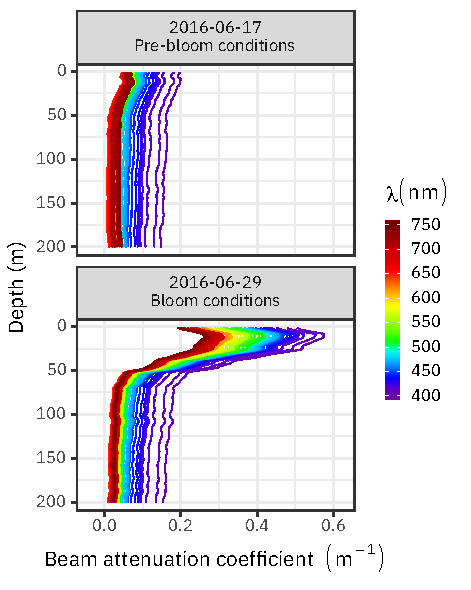
\includegraphics[scale = 2]{../../../graphs/fig5.pdf}
	\caption{Beam attenuation coefficients ($c$, m\textsuperscript{-1}) measured in 2016 using an ACS before and during the phytoplankton bloom. Note that the colors of the lines correspond to wavelength frequencies.}
\end{figure}

\clearpage
\newpage

\begin{figure}[h]
	\centering
	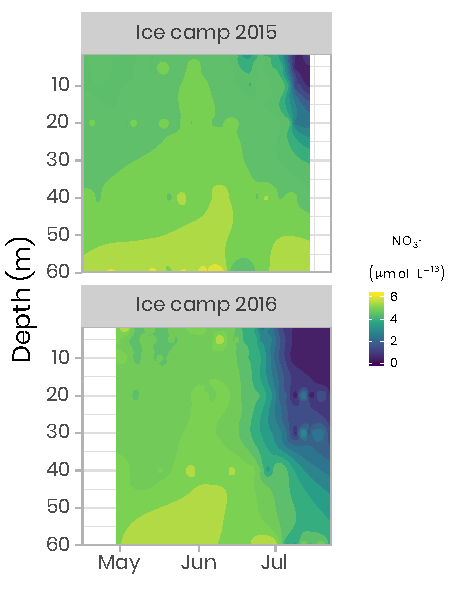
\includegraphics[scale = 2]{../../../graphs/fig6.pdf}
	\caption{Temporal evolution of the nitrates in the first 60 m of the water column for both ice camp missions.}
\end{figure}

\clearpage
\newpage

\begin{figure}[h]
	\centering
	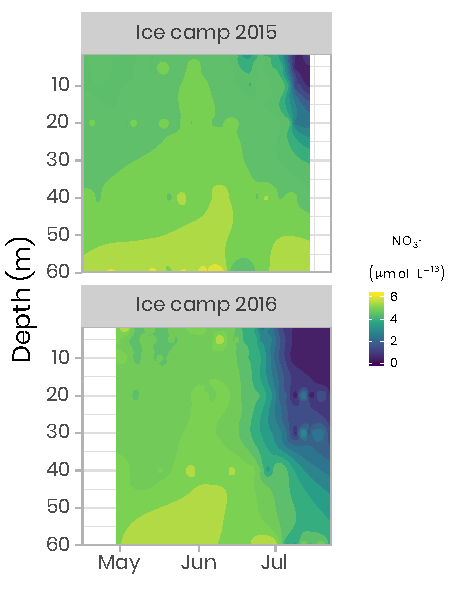
\includegraphics[scale = 2]{../../../graphs/fig7.pdf}
	\caption{Temporal evolution of chlorophyll a in ice and water (depth-integrated) for both ice camp missions. Note that the water chlorophyll a have been integrated over the first 100 m of the water column whereas the ice chlorophyll a was measured on the bottom 0-10 cm of the ice cores.}
\end{figure}

\end{document}
